\documentclass[a4paper]{article}
\usepackage[UTF8]{ctex}
\usepackage{geometry}
\usepackage{graphicx}
\usepackage{url}
\usepackage{multirow}
\usepackage{array}
\usepackage{booktabs}
\usepackage{url}
\usepackage{enumitem}
\usepackage{graphicx}
\usepackage{float}
\usepackage{amssymb}
\usepackage{amsmath}
\usepackage{subfig}
\usepackage{longtable}
\usepackage{pifont}
\usepackage{color}

\allowdisplaybreaks

\geometry{a4paper, scale=0.78}

% \begin{figure}[H]
%     \centering
%     \includegraphics[width=.55\textwidth]{E.png}
%     \caption{矩阵与列向量的乘法}
%     \label{fig:my_label_1}
% \end{figure}

% \left\{
% \begin{array}{ll}
%       x+2x+z=2 & \\
%       3x+8y+z=12 & \\
%       4y+z=2
% \end{array}
% \right.

% \begin{enumerate}[itemindent = 1em, itemsep = 0.4pt, parsep=0.5pt, topsep = 0.5pt]

% \end{enumerate}

%\stackrel{a}{\longrightarrow}

\title{Support Vector Machine 01 Hard Margin Modeling and Solution}
\author{Chen Gong}
\date{13 November 2019}

\begin{document}
\maketitle

众所周知,Support Vector Machine (SVM)有三宝,间隔,对偶,核技巧。所以,SVM可以大致被分为三类:hard-margin SVM;soft-margin SVM;kernel SVM。

\section{SVM基本思想}
\begin{figure}[H]
    \centering
    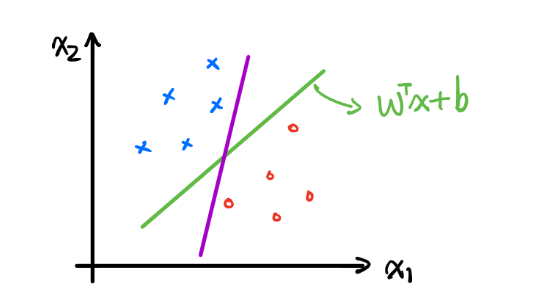
\includegraphics[width=.55\textwidth]{微信图片_20191113104442.png}
    \caption{二分类问题模型图}
\end{figure}

支持向量机模型可以被简要的描述为:$f(w) = w^Tx + b$。很显然这是一个判别模型。实际上,我们想一想就知道,这样的直线其实有很多的。但是紫色的那条虽然可以做到分类的效果,但是效果也太差了,没有什么鲁棒性,泛化能力并不行。显然,绿色的那条直线要更好一些。那么,SVM的基本思想可以被简要的概述为,找到一条最好的直线,离样本点距离足够的大。

\section{SVM模型建立}
数据集可以描述为$D=\{(x_i,y_i)\}^{N}_{i=1}$,其中$x_i\in\mathbb{R}^{p}$,$y_i\in\{1,-1\}$。

首先我们希望,把这些点的间隔分得越大越好,并且根据符号函数给不同的值相应的类别标号。那么,我们可以写做:
\begin{equation}
    \begin{split}
        & \max_{w,b} \ margin\ (w,b) \\
        & s.t. 
        \left\{
        \begin{array}{ll}
            w^Tx_i+b>0 & y_i = +1 \\
            w^Tx_i+b<0 & y_i = -1 \\
        \end{array}
        \right.
    \end{split}
\end{equation}

由于$y_i$和$w^T_ix+b$是同号的,那么很显然有$y_i(w^T_ix+b)>0$,所以,模型被我们改写为:
\begin{equation}
    \begin{split}
        & \max_{w,b} \ margin\ (w,b) \\
        & s.t.\quad y_i(w^T_ix+b)>0 \quad (i = 1,2,\cdots,N)
    \end{split}
\end{equation}

平面上一点到某一直线的矩阵的计算方法比较简单。对于平面上一条直线$y=w^Tx+b$,点$(x_i,y_i)$到直线的距离,可以被记做:
\begin{equation}
    distance = \frac{1}{||w||}|w^Tx+b|
\end{equation}

我们的希望是离超平面最近的点分得越开越好。离超平面最近的点就是$\min distance(w,b,x_i)$,这个是针对点$x_i (i=1,2,\cdots,n)$。然后就是分得越开越好,那么我们可以描述为$\max \min distance(w,b,x_i)$,这个是针对$w,b$进行优化的。那么我们可以把模型进一步改写为:
\begin{equation}
    \begin{split}
        & \max_{w,b} \min_{x_i} \frac{1}{||w||}|w^Tx_i+b| \\
        & s.t.\quad y_i(w^T_ix+b)>0 \quad (i = 1,2,\cdots,N)
    \end{split}
\end{equation}

对于约束条件$y_i(w^T_ix+b)>0 \quad (i = 1,2,\cdots,N)$,很显然可以得到$\exists \gamma > 0$使得$s.t.\ \min y_i(w^T_ix+b)=\gamma$。这里很显然我们可以使用一个小技巧来做一些的调整,来使我们方便计算,我们可以把约束条件转换为$s.t.\ \min \frac{y_i(w^T_ix+b)}{z}=\frac{\gamma}{z}$。我们很显然可以看到,$w$和$b$之间是可以自由放缩的,那么就放缩到令$\frac{\gamma}{z}=1$,那么就有$\min y_i(w^T_ix+b)=1$。于是,模型可以化简为:
\begin{equation}
    \begin{split}
        & \max_{w,b} \frac{1}{||w||} \\
        & s.t.\quad \min_{x_i} y_i(w^T_ix+b)=1 \Longrightarrow y_i(w^T_ix+b)\geq 1 \quad (i = 1,2,\cdots,N)
    \end{split}
\end{equation}

将该优化问题进行等价变换:
\begin{equation}
    \begin{split}
        & \min_{w,b} \ \frac{1}{2} w^Tw \\
        & s.t. \quad y_i(w^T_ix+b)\geq 1 \quad (i = 1,2,\cdots,N)
    \end{split}
\end{equation}

很显然,这是一个凸优化 (Convex Optimization)问题,目标函数是二次函数,一共有$N$个约束。那么这是一个二次规划问题 (Quadratic Programming),通常也被描述为QP问题。

\section{模型求解}
在支持向量机的模型求解中,一个非常重要的概念就是将原问题(Prime Problem)转换为对偶问题(Dual Problem)。我们将模型进一步改写为:
\begin{equation}
    \begin{split}
        & \max_{w,b} \ \frac{1}{2} w^Tw \\
        & s.t. \quad 1-y_i(w^T_ix+b)\leq 0 \quad (i = 1,2,\cdots,N)
    \end{split}
\end{equation}

求解带约束的极值,显然需要采用拉格朗日乘子法,我们定义拉格朗日函数为:
\begin{equation}
    \mathcal{L}(w,b,\lambda) = \frac{1}{2}w^Tw + \sum_{i=1}^N\lambda_i(1-y_i(w^Tx_i+b))
\end{equation}

在拉格朗日数乘法里,$\lambda$一定是大于零的数。所以模型为:
\begin{equation}
    \begin{split}
        & \min_{w,b} \ \max_\lambda \ \mathcal{L}(w,b,\lambda) \\
        & s.t. \quad \lambda_i \geq 0 \quad (i = 1,2,\cdots,N)
    \end{split}
\end{equation}

很显然,在这里,{\color{red} 我们就将一个带约束的问题转换成了一个无约束的问题。}

然而我们需要考虑一个问题,那就是$\mathcal{L}(w,b,\lambda)$是否一定和公式(7)等价呢?这需要探究验证一下。
\begin{equation}
    \begin{split}
        & if \ 1-y_i(w^Tx_i+b)\geq 0,\ \max_\lambda\mathcal{L}(\lambda,w,b)=+\infty \\
        & if \ 1-y_i(w^Tx_i+b)\leq 0,\ \max_\lambda\mathcal{L}(\lambda,w,b)=0 \\
    \end{split}
\end{equation}

很显然在$\min_{w,b} \ \max_\lambda \ \mathcal{L}(w,b,\lambda)$的计算中可以表示为:
\begin{equation}
    \min_{w,b} \ \max_\lambda \ \mathcal{L}(w,b,\lambda) = \min_{w,b}\{ +\infty,\frac{1}{2}w^Tw \} = \frac{1}{2}w^Tw
\end{equation}

所以在上述的描述中,我们可以得到,实际上$\min_{w,b} \ \max_\lambda \ \mathcal{L}(w,b,\lambda)$中隐藏了一个$1-y_i(w^Tx_i+b)\leq 0$的隐藏条件。所以两种写法实际上是等价的。为了方便计算,下面我们需要使用对偶的方法,也就是将模型作如下的转换:
\begin{equation}
    \left\{
    \begin{array}{ll}
          \min_{w,b} \ \max_\lambda \ \mathcal{L}(w,b,\lambda) & \\
          s.t.\quad \lambda_i \geq 0 & \\
    \end{array}
    \right.
    \stackrel{dual}{\Longrightarrow}
    \left\{
    \begin{array}{ll}
          \max_\lambda \ \min_{w,b} \ \mathcal{L}(w,b,\lambda) & \\
          s.t.\quad \lambda_i \geq 0 & \\
    \end{array}
    \right.
\end{equation}

这里我们需要介绍两种对偶关系,所谓:

弱对偶关系就是:$\min\max\mathcal{L} \geq \max\min\mathcal{L}$。

强对偶关系就是:$\min\max\mathcal{L} = \max\min\mathcal{L}$。

大家或许对这个关系会有点懵逼,其实仔细用直觉来想想还是很好接受的,具体的证明过程这里就不再做过多的阐述了。中国有句古话叫:“宁做鸡头不做凤尾”,但是凤就是凤始终要比鸡好。先取$\max$就是凤的意思,然后取$\min$就是凤尾。同理先取$\min$就是鸡的意思,然后取$\max$就是鸡头的意思。凤尾肯定比鸡头要好,当然这是直观的理解。而对于强对偶关系,需要我们满足KKT条件,这个后面会详细的说。

\subsection{估计参数的值}
我们的目标是$\min_{w,b} \ \mathcal{L}(w,b,\lambda)$,那么
\begin{equation}
    \frac{\partial \mathcal{L}}{\partial b} = \frac{\partial}{\partial b}\sum_{i=1}^N
    \lambda_i[1-y_i(w^Tx_i+b)] = 0
\end{equation}
\begin{equation}
    -\sum_{i=1}^N \lambda_iy_i = 0
\end{equation}

代入到$\mathcal{L}(w,b,\lambda)$中可得,
\begin{align}
    \mathcal{L}(w,b,\lambda) = & \frac{1}{2}w^Tw + \sum_{i=1}^N\lambda_i(1-y_i(w^Tx_i+b)) \\
    = & \frac{1}{2}w^Tw + \sum_{i=1}^N\lambda_i - \sum_{i=1}^N\lambda_iy_iw^Tx_i - \sum_{i=1}^N\lambda_iy_ib \\
    = & \frac{1}{2}w^Tw + \sum_{i=1}^N\lambda_i - \sum_{i=1}^N\lambda_iy_iw^Tx_i
\end{align}

下一步,则是对$w$求偏导,
\begin{equation}
    \frac{\partial \mathcal{L}}{\partial w} 
    = \frac{\partial }{\partial w}[\frac{1}{2}w^Tw + \sum_{i=1}^N\lambda_i - \sum_{i=1}^N\lambda_iy_iw^Tx_i]
    = w - \sum_{i=1}^N\lambda_iy_ix_i = 0 
\end{equation}

解得:
\begin{equation}
    w = \sum_{i=1}^N\lambda_iy_ix_i 
\end{equation}

将$w$的值代入到$\mathcal{L}(w,b,\lambda)$中可以得到:
\begin{equation}
    \begin{split}
        \mathcal{L}(w,b,\lambda) = & \frac{1}{2}(\sum_{i=1}^N\lambda_iy_ix_i)^T(\sum_{i=1}^N\lambda_iy_ix_i) + \sum_{i=1}^N\lambda_i - \sum_{i=1}^N\lambda_iy_i(\sum_{i=1}^N\lambda_iy_ix_i)^Tx_i \\
        = & \frac{1}{2}\sum_{i=1}^N\sum_{j=1}^N\lambda_i\lambda_jy_iy_j(x_i^Tx_j) - \sum_{i=1}^N\sum_{j=1}^N\lambda_i\lambda_jy_iy_j(x_j^Tx_i) + \sum_{i=1}^N\lambda_i \\
        = & -\frac{1}{2}\sum_{i=1}^N\sum_{j=1}^N\lambda_i\lambda_jy_iy_j(x_i^Tx_j) + \sum_{i=1}^N\lambda_i \\
    \end{split}
\end{equation}

所以,模型被我们改写为:
\begin{equation}
    \left\{
    \begin{array}{ll}
          \max_\lambda -\frac{1}{2}\sum_{i=1}^N\sum_{j=1}^N\lambda_i\lambda_jy_iy_j(x_i^Tx_j) + \sum_{i=1}^N\lambda_i & \\
          s.t.\quad \ \lambda_i \geq 0,\ \sum_{i=1}^N \lambda_iy_i = 0  & \\
    \end{array}
    \right.
\end{equation}

\section{KKT条件}
这个KKT条件或许会让很多人都感觉一脸懵逼,作者自己也理解了很久才勉强把它看懂的,如果有什么不到位的地方,欢迎发邮件到gongchen2020@ia.ac.cn与作者取得联系。深刻理解KKT条件需要掌握一些凸优化的知识,支持向量机是一个典型的凸二次优化问题。KKT条件可以帮助我们理解支持向量机的精髓,什么是支持向量?支持向量机只需要用少量的数据,有很强的鲁棒性,并且可以取得很好的效果。

KKT条件可以描述为:
\begin{equation}
    \left\{
    \begin{array}{ll}
          \frac{\partial \mathcal{L}}{\partial w} = 0,\quad
          \frac{\partial \mathcal{L}}{\partial b} = 0 & \\
          \lambda_i(1-y_i(w^Tx_i+b)) = 0 & \\
          \lambda_i \geq 0 & \\
          1-y_i(w^Tx_i+b) \leq 0 
    \end{array}
    \right.
\end{equation}

其中$\lambda_i(1-y_i(w^Tx_i+b)) = 0$是互补松弛条件(Complementary Relaxation Condition)。{\color{red} 满足KKT条件是原问题的对偶(dual)问题有强对偶关系的充分必要条件。}下面我们用一张图来进行理解KKT条件的作用:
\begin{figure}[H]
    \centering
    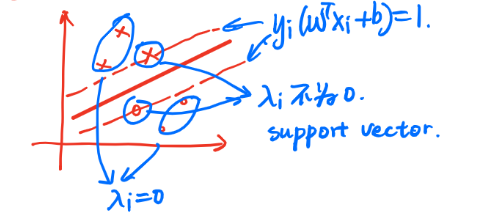
\includegraphics[width=.55\textwidth]{微信图片_20191114112701.png}
    \caption{支持向量的KKT条件}
    \label{fig:my_label_1}
\end{figure}

首先,需要明确,离分界面最近的数据点满足这个条件,$y_i(w^Tx_i+b)=1$至于为什么?前面的公式(4)有详细的分析。那么离分界面最近的数据点就被我们称为支持向量了。在支持向量上$1-y_i(w^Tx_i+b)=0$,那么$\lambda_i$可以不为0。而在其他向量上一定会有$1-y_i(w^Tx_i+b)<0$为了满足$\lambda_i(1-y_i(w^Tx_i+b)) = 0$,必然有$\lambda_i=0$,那么我们就可以理解为这个数据点失去了作用。所以,KKT条件使得,支持向量机中只有支持向量在模型的优化中有作用,这实在是太棒了。

为了确定这个超平面,我们已经得到了
\begin{equation}
    w^\ast = \sum_{i=1}^N \lambda_iy_ix_i
\end{equation}

但是,现在怎么求$b^\ast$是一个很尴尬的问题,因为我们在求$\frac{\partial \mathcal{L}}{\partial b}$的时候,并没有看到和$b$相关的等式。但是我们知道只有支持向量会在模型求解中起作用,那么有支持向量$(x_k,y_k)$使得$1-y_k(w^Tx_k+b)=0$。所以:
\begin{gather}
    y_k(w^Tx_k + b) = 1 \\
    y_k^2(w^Tx_k + b) = y_k \\
    b^\ast = y_k - w^Tx_k = y_k - \sum_{i=1}^N \lambda_iy_ix_i^T x_k
\end{gather}

那么做到这里,我们的hard-margin SVM就已经做完了。模型为$f(x)=sign(w^{\ast T}x+b^{\ast})$,超平面为$w^{\ast T}+b^{\ast}$。其中$w^\ast = \sum_{i=1}^N \lambda_iy_ix_i$,$b^\ast = y_k - \sum_{i=1}^N \lambda_iy_ix_i^T x_k$。

\section{小结}
本节主要探究了Hard-margin SVM的建模和求解。最终解得对于一个$\{ (x_i,y_i)_{i=1}^N \}$的分类问题,使用支持向量机来求解,我们可以得到,分类模型为:
\begin{equation}
    f(x)=sign(w^{\ast T}x+b^{\ast}) \qquad
    \left\{
    \begin{array}{ll}
         w^\ast = \sum_{i=1}^N \lambda_iy_ix_i & \\
         b^\ast = y_k - \sum_{i=1}^N \lambda_iy_ix_i^T x_k & \\
    \end{array}
    \right.
\end{equation}

KKT条件是原问题的对偶(dual)问题有强对偶关系的充分必要条件。它成功的使支持向量机模型的求解只和支持向量有关,这也是支持向量机的强大之处,运算比较简单,而且具有较强的鲁棒性。
\begin{equation}
    \left\{
    \begin{array}{ll}
          \frac{\partial \mathcal{L}}{\partial w} = 0,\quad
          \frac{\partial \mathcal{L}}{\partial b} = 0,\quad
          \frac{\partial \mathcal{L}}{\partial \lambda} = 0 & \\
          \lambda_i(1-y_i(w^Tx_i+b)) = 0 & \\
          \lambda_i \geq 0 & \\
          1-y_i(w^Tx_i+b) \leq 0 
    \end{array}
    \right.
\end{equation}














\end{document}